\chapter{D3.js – Data-Driven Documents}
\label{cha:d3js}

Chapter \ref{cha:d3js} provides an overview of the popular JavaScript library D3 which is used to simplify implementations of any data visualizations in the web for developers. It not only provides an overview of the libraries beginnings but also goes into detail about how to implement projects with D3. The knowledge is required to understand the performance comparisons in chapter \ref{cha:performance} and \ref{cha:conclusion}.

%% ------------------------------------------------------------------------------------------- %%
%% ------------------------------------------------------------------------------------------- %%
%% ------------------------------------------------------------------------------------------- %%

\section{Introduction to D3}

D3 is a JavaScript library that helps developers create highly sophisticated data visualizations on the web via a universal tool that is platform agnostic: the browser. The official documentation of D3 in \cite{D3Website} explains the library as a toolkit, that allows binding data to the DOM. Also, it gives an overview of the vast amount of helpful tools that can be used to visualize data. The library includes all kinds of functionality, ranging from simple array and mathematic operations to complex simulations, that are calculated in real time.

Some of the most popular features of D3 is to render user interactable animated charts. Not only is it possible to easily create a bar chart for instance, but all other kinds of charts as well. A full list of available packages can be found in \cite{D3Github}. The library is prevalent amongst data scientists as it is quite easy to create complex data visualizations in the web quickly.

D3 also provides some other utility functions that can be useful in many use-cases. There is, for example, a module, that calculates chromatic colors for charts to get colors that have the maximum diversity to each other to be easily distinguishable as seen in \cite[/d3-scale-chromatic]{D3Github}. Another example in \cite[/d3-array]{D3Github} shows, that the library also provides some useful array manipulating functions which come in handy when having to deal with big data sets. Also generating random numbers via various distributions is no problem when using the d3-random package in \cite[/d3-random]{D3Github}. The list of useful data manipulation tools goes on and dealing with every aspect of the library would go far beyond the scope of this paper. 

What makes D3 unique though is the possibility to create individual data structures for rendering sophisticated data visualizations. The library provides scatter plots in \cite[/d3-scale]{D3Github} or pie charts, line charts, area charts, radial bar charts, tree maps in \cite[/d3-shape]{D3Github} to name a few. D3 also provides utility functions to add labels or user interaction to each mentioned and not mentioned data visualization type. Also, a significant advantage of using D3 is, that it also provides simple methods to transform any D3 visualization into being user interactable by creating floating tooltips or sliders, switches, or knobs, which control the visualization.

Due to the immense size of the library and its many data manipulation tools, D3 is divided into different sub-modules to prevent users of the library having to download the full library code bundle in the browser to be able to use the library. \cite{D3Github} shows a full list of every available tool that can be used in composition with the base package of D3. When using D3 in a big production project, all modules can be integrated into any project via using nodes package manager npm and download it from its registry\footnote{https://www.npmjs.com/search?q=d3}.

\begin{emergency}{1em}
There are multiple examples on the documentation's example page in \cite{D3Examples} which show what developers can achieve by using the D3 library. The API documentation is a comprehensive documentation of the complete feature set of D3 as seen in \cite[\mbox{/d3/blob/master/API.md}]{D3Github}.
\end{emergency}

%% ------------------------------------------------------------------------------------------- %%
%% ------------------------------------------------------------------------------------------- %%
%% ------------------------------------------------------------------------------------------- %%

\section{Explaining the D3 API} 

This section aims to discuss the most vital aspects of the D3's API to understand code samples, that are presented in later chapters. Some general knowledge of D3's API is of utmost importance as the knowledge is crucial for understanding the comparisons of React and D3 in chapter \ref{cha:visualization}. As mentioned before, the D3 API mostly consists of consecutive chained imperative function calls, that manipulate the visualization data and binds it to the DOM. \cite[P.\ 625]{prgLngDesignImpl} describes the imperative programming pattern as a static division of a program into its concurrent tasks which means, that the programmer uses statements to change the programs state. 

According to the documentation in \cite{D3Github} the library D3 was created in 2010. Thus it can be noticed, that the libraries API originates from a time, where developers did not even think about using JavaScript in productive or even enterprise environments. Therefore large codebases written with D3 tend to be hardly scalable and difficult to maintain. Multiple instruction function calls in \ref{prog:d3selection} show, that D3 code is indeed imperative. Also, the library makes use of a software pattern called ''chaining''. The pattern works because each function returns an instance of itself to enable the addition of an infinite amount of functions that can be added to the chain.

\begin{program}
\caption{D3 selection, enter, and exit example}
\label{prog:d3selection}
\begin{JsCode}
// earlier in the script

const svg = d3.select('.container')  
const node = svg.selectAll('.node')

// handling data changes of the simulation

node
  .exit()
  .style('fill', '#b26745')
  .transition(t)
  .attr('r', 1e-6)
  .remove()

node
  .transition(t)
  .style('fill', '#3a403d')
  .attr('r', (node) => node.size)

node = node
  .enter()
  .append('circle')
  .style('fill', '#45b29d')
  .attr('r', (node) => node.size)
  .attr('id', (node) => node.name)
\end{JsCode}
\end{program}

\begin{program}
\caption{Negative example of how confusing and unmaintainable D3 code can get}
\label{prog:d3confusing}
\begin{JsCode}
d3.select(_this).classed('active', true)
d3.select(_this)
  .select('.circle')
  .transition(500)
  .attr('stroke', function(d) {
    if (d.rings && d.rings.length > 0) return '#404348'
    return d.color || COLORS[d.type.toUpperCase()] || '#27292c'
  })
  .attr('fill', function(d) {
    return '#404348'
  })
  .style('filter', 'drop-shadow(0 3px 4.7px rgba(0,0,0,.54))')
d3.select(_this)
  .selectAll('.ring')
  .transition(500)
  .attr('opacity', 1)
d3.select(_this)
  .selectAll('.node-background')
  .transition(500)
  .attr('opacity', 0)
d3.select(_this)
  .selectAll('.sub-circle')
  .transition(500)
  .attr('cx', function(d, i) {
    let deg = ((Math.PI * 2) / 8) * i - Math.PI
    let x = Math.sin(deg)
    let offset = event.rings ? event.rings.length * 15 : 0
    return x * (d.r + 5 + offset)
  })
  .attr('cy', (d, i) => {
    let deg = ((Math.PI * 2) / 8) * i - Math.PI
    let y = Math.cos(deg)
    let offset = event.rings ? event.rings.length * 15 : 0
    return y * (d.r + 5 + offset)
  })
  .attr('stroke', '#FFF')
\end{JsCode}
\end{program}

Selecting DOM nodes and creating a D3 selection model is, therefore, a vital aspect of D3's API. Via selection D3 can connect JavaScript application data to actual DOM nodes as \cite[/d3-selection]{D3Github} shows. An example can be seen in \ref{prog:d3selection}. Because the library is imperative, each node that is added or removed is handled via a chained function call as the append function in \ref{prog:d3selection} shows very well. When adding or removing multiple DOM nodes and the individual nodes of the simulation are complicated DOM structures, the code quickly gets very incomprehensive as demonstrated in \ref{prog:d3confusing}. The provided example in \ref{prog:d3selection} only appends one simple circle element for instance though in comparison to the much more complicated example in \ref{prog:d3confusing}. 

Not only is it possible to select DOM nodes via D3 but the library also contains the feature of selecting entering and exiting nodes as lines 9 and 21 showcase in \ref{prog:d3selection}. The enter and exit selection function calls can be used to explicitly handle nodes that enter and exit the visualiization according to the data that is bound to the DOM. The chained function calls can then handle the enter and exit selections accordingly. Line 21 in \ref{prog:d3selection} shows an enter selection which appends a circle svg element for each new data object and also applies various attributes and a style.

When the data of a visualization changes, some nodes might be deleted, some new nodes might appear but some nodes might also stay in the visualization but change their position. D3 covers that use-cases by including the possibility to add transitions to node selections. The transition feature lets developers specify how to handle DOM elements that stay in the visualization if the data is updated. Advanced animations and transitions can be added via a simple function call. Line 8 in \ref{prog:d3selection} for example shows a selection where all nodes are selected that are removed after the data has changed. Furthermore the color is changed and a transition is added, which transforms the radius attribute of the node until it reaches the specified amount, 1e-6 in this case. Finally the node is then removed completely from the DOM resulting in a nice animation of the node exiting the visualization.

The code in \ref{prog:d3selection} also clearly shows, that every attribute and style instruction of and added DOM nodes have to be handled via a chained function call. On line 23 in \ref{prog:d3selection} the \texttt{fill} property is added to the \texttt{<circle>} SVG element. Each additional style property would require a consecutive call of the \texttt{style('property', [style])} function.

Also, a key component of D3's API is the possibility to pass attribute handling functions instead of hardcoded values. Those computed properties can be found in line 24 and 25 in \ref{prog:d3selection}. By passing a function to property or attribute setters like the \texttt{.style('attribute', [style])} method, the passed handler is called by D3 as a callback by providing each node's data to the callback. When rendering 10 nodes, the attribute function on line 24 in \ref{prog:d3selection} which sets the radius of the node would, therefore, be called 10 times as well, setting the radius for each specific node individually.

The code example \ref{prog:d3confusing} is taken from production code and shows how hard to read D3 code can get if multiple DOM changes have to be handled imperatively. Not only the addition of the nodes has to be handled via function calls, but also some general node properties like CSS styles or custom attributes.

Over the years better software patterns emerged and experience shows, that chaining is a software pattern that was new at the time but can cause code that is hard to maintain. Nowadays this library would probably be written with a functional approach, letting developers compose their simulations via functional composition as various libraries and frameworks on the internet already do. The problem with the example \ref{prog:d3selection} is that the code cannot be reused, as it is hardcoded into the chain. Nowadays many frameworks for building frontend applications use a declarative approach for binding the view to the data model. More information about declarative approaches can be found in chapter \ref{cha:react}. D3's API still uses the imperative software pattern which forces developers to chain library function statements to control multiple elements in the DOM.

%Chaining is not the only problem that might decrease the code quality of a project. The other problem of D3 is, %that handling DOM nodes is not declarative but imperative code as well. 

%% ------------------------------------------------------------------------------------------- %%
%% ------------------------------------------------------------------------------------------- %%
%% ------------------------------------------------------------------------------------------- %%

\begin{figure}
  \centering
  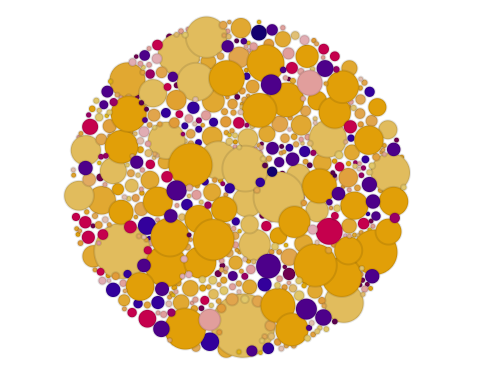
\includegraphics[width=0.5\columnwidth]{force001.PNG}
  \caption{The force graph with default center force. All nodes are attracted to the same center without overlapping each other.}
  \label{fig:force001}
\end{figure}

\begin{figure}
  \centering
  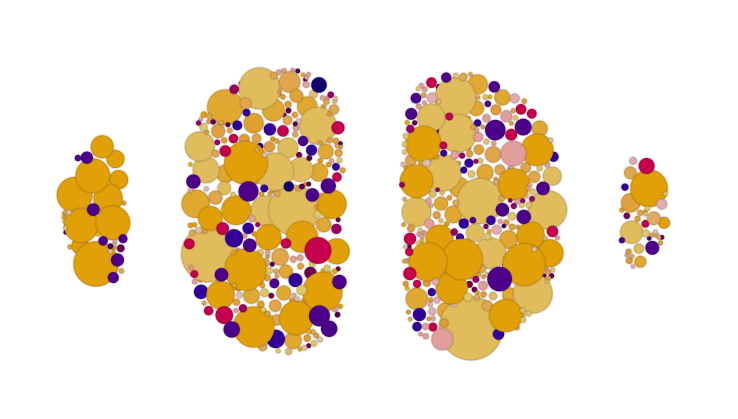
\includegraphics[width=0.6\columnwidth]{force002.PNG}
  \caption{A sample force graph with more than one center force. Having more than one force centers means that different nodes are attracted to their assigned center force.}
  \label{fig:force002}
\end{figure}

\section{Force Graphs -- Real time rendered data visualizations}

Due to the immense size of D3, the focus of this thesis and its project lies on a rather ''small'' but quite important part of the library -- the force graph simulation. It is the graph type that is integrated into React as showcased by the thesis project. The visualizations consist of objects that interact with each other in a two-dimensional space. By interacting and moving objects all other objects in the animation are also affected. Figures \ref{fig:force001} and \ref{fig:force002} show an example of D3's force simulation. In figure \ref{fig:force001} there is a single center force that keeps all nodes in the center but also keeps individual nodes from overlapping each other. Force graphs can also be configured to make nodes reject each other even further than their actual size as figure \ref{fig:force004} shows. It is also possible to implement so-called links, that also add some complexity to the simulation, as nodes are dependent on each other and not only reject each other but also attract linked nodes as figure \ref{fig:force002} and \ref{fig:force005} shows.

As previously mentioned, all force simulations are calculated, animated, and rendered in the browser which also includes user interaction. The user can for example drag nodes around which of course then affect other nodes and the whole simulation as well. Figure \ref{fig:force003} shows well, how dragging one node affects the whole force graph, as all connected nodes follow the dragged node while still rejecting each other and while being attracted to the center force.

\begin{figure}
  \centering
  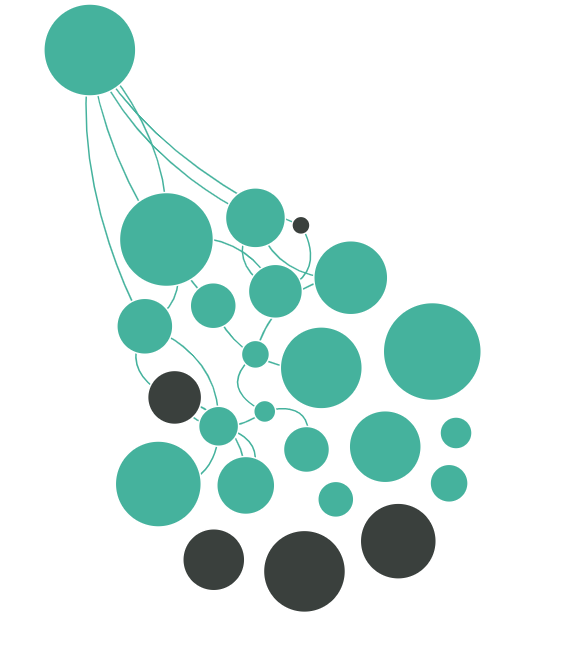
\includegraphics[width=0.4\columnwidth]{forceOwn002.PNG}
  \caption{A sample force graph where the top node is dragged up to the left and the other nodes are dragged along. The force is still keeping the other nodes apart and also drawn to the center though.}
  \label{fig:force003}
\end{figure}

\begin{figure}
  \centering
  
\includegraphics[width=0.45\columnwidth]{forceOwn003.PNG}
  \caption{A sample force graph with one center force. The nodes are configured to reject each other with the function \texttt{r+r/2}}
  \label{fig:force004}
\end{figure}

D3 provides a somewhat simplified API to be able to quickly implement force graphs in the browser as it can be read in \cite[/d3-force/blob/master/README.md]{D3Github}. The way force simulations work is that developers first have to define or build the simulation. There is a factory method as seen in line 1 of \ref{prog:simulation} which takes the nodes of the graph as an argument and builds a default simulation. The nodes have to be provided in a particular scheme so D3 can correctly parse the node array. 

\begin{program}
\caption{Code snippets for D3 force simulation code}
\label{prog:simulation}
\begin{JsCode}
simulation.forceSimulation([nodes]) // factory method for a standard force simulation
simulation.tick([iterations]) // called on every tick the simulation goes through
simulation.start() // starts a stopped simulation
simulation.stop() // stops a started simulation
simulation.restart() // restarts a simuliation, resets alpha
simulation.alpha([alpha]) // directly sets alpha value
simulation.alphaTarget([alphaTarget]) // sets alpha target value
\end{JsCode}
\end{program}

\begin{program}
\caption{Sample initialization of a D3 force graph}
\label{prog:d3forceinit}
\begin{JsCode}
const simulation = forceSimulation(data)
  .force('charge', forceManyBody().strength(-150))
  .force('forceX', forceX().strength(0.1))
  .force('forceY', forceY().strength(0.1))
  .force('center', forceCenter())
  .alphaTarget(1)
  .on('tick', ticked)
\end{JsCode}
\end{program}

Another very important aspect of force graphs is the so called ''alpha'' value system as documented in \cite[/d3-force/blob/master/README.md]{D3Github}, which controls how long the simulation lives. The alpha valueis a gradually decaying value that makes the simulation stop if a certain value is reached. Every simulationhas a function that is called every ''tick'' of the simulation as shown in line 2 of \ref{prog:simulation}. Everytick the alpha value decays via a predefinable function, it happens logarithmically per default. The tickingfunction takes a handling function will be passed every node position in the simulation which then letsdevelopers link the data to the DOM with D3 again. The tick function will be very important lateron when thecombination of D3 and React is explained in more detail. \ref{prog:d3forceinit} is a simple example that shows how to initialize a D3 force simulation.

\begin{figure}
  \centering
  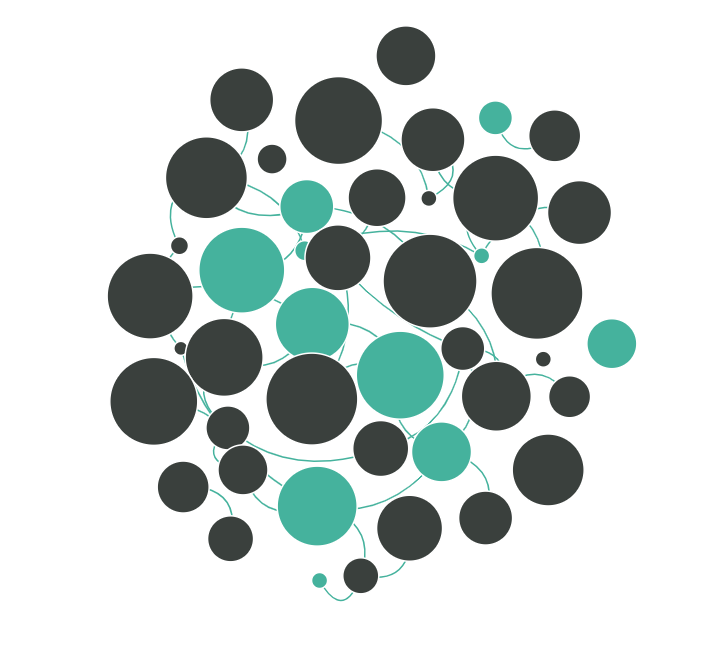
\includegraphics[width=0.45\columnwidth]{forceOwn001.PNG}
  \caption{A sample force graph where some nodes are linked together while still rejecting each other;}
  \label{fig:force005}
\end{figure}

If there is a user interaction, the simulation sometimes has to be restarted or reheated. Programmers can set alpha values and targets to reheat or restart the simulation in case a node is dragged by the user which would possibly require many other nodes in the simulation to react to that user input. That way also the speed of the simulation can be controlled via setting a custom decay function. The documentation in \cite[/d3-force/blob/master/README.md]{D3Github} points to a few methods that can achieve said functionality. The functions on line 3, 4, and 5 of \ref{prog:simulation} can be used to reheat a simulation. Also the functions in line 6 and 7 of \ref{prog:simulation} can be used to set values directly to alter the simulation's life span.

\begin{program}
\caption{D3 written in a fictional functional way}
\label{prog:d3functional}
\begin{JsCode}
const forceParams = compose(
  force('charge', pipe(forceManyBody(), strength(-150))),
  force('forceX', pipe(forceX(), strength(0.1))),
  force('forceY', pipe(forceY(), strength(0.1))),
  force('center', forceCenter()),
)

const simulation = compose(
  forceParams,
  alphaTarget(1),
  on('tick', ticked),
  forceSimulation
)(data)
\end{JsCode}
\end{program}

If a functional approach would be used the code from \ref{prog:d3forceinit} would look more like in example \ref{prog:d3functional}. The difference between the two code examples in \ref{prog:d3forceinit} and \ref{prog:d3functional} might appear to be very subtle, but in reality, it is very significant. By looking closer, it is clear, that the variable \texttt{forceParams} is a functional composition of methods, that can be reused multiple times in the application. In the first example in \ref{prog:d3forceinit} the simulation configuration is locked in the function chain. Chaining is a pattern which can easily cause duplicated code in any codebase. 

Writing functional D3 code could also alleviate the confusing unmaintainable code in \ref{prog:d3confusing} as developers can easily compose repeating DOM manipulation sequences and reuse them throughout the codebase without having to touch code on multiple files in case there is a bug that effects multiple aspects of the application.
